\section{Chain-of-Thought-Guided Retrieval and Open-Domain QA}
\label{sec:method}

\begin{figure*}[!ht]
\centering
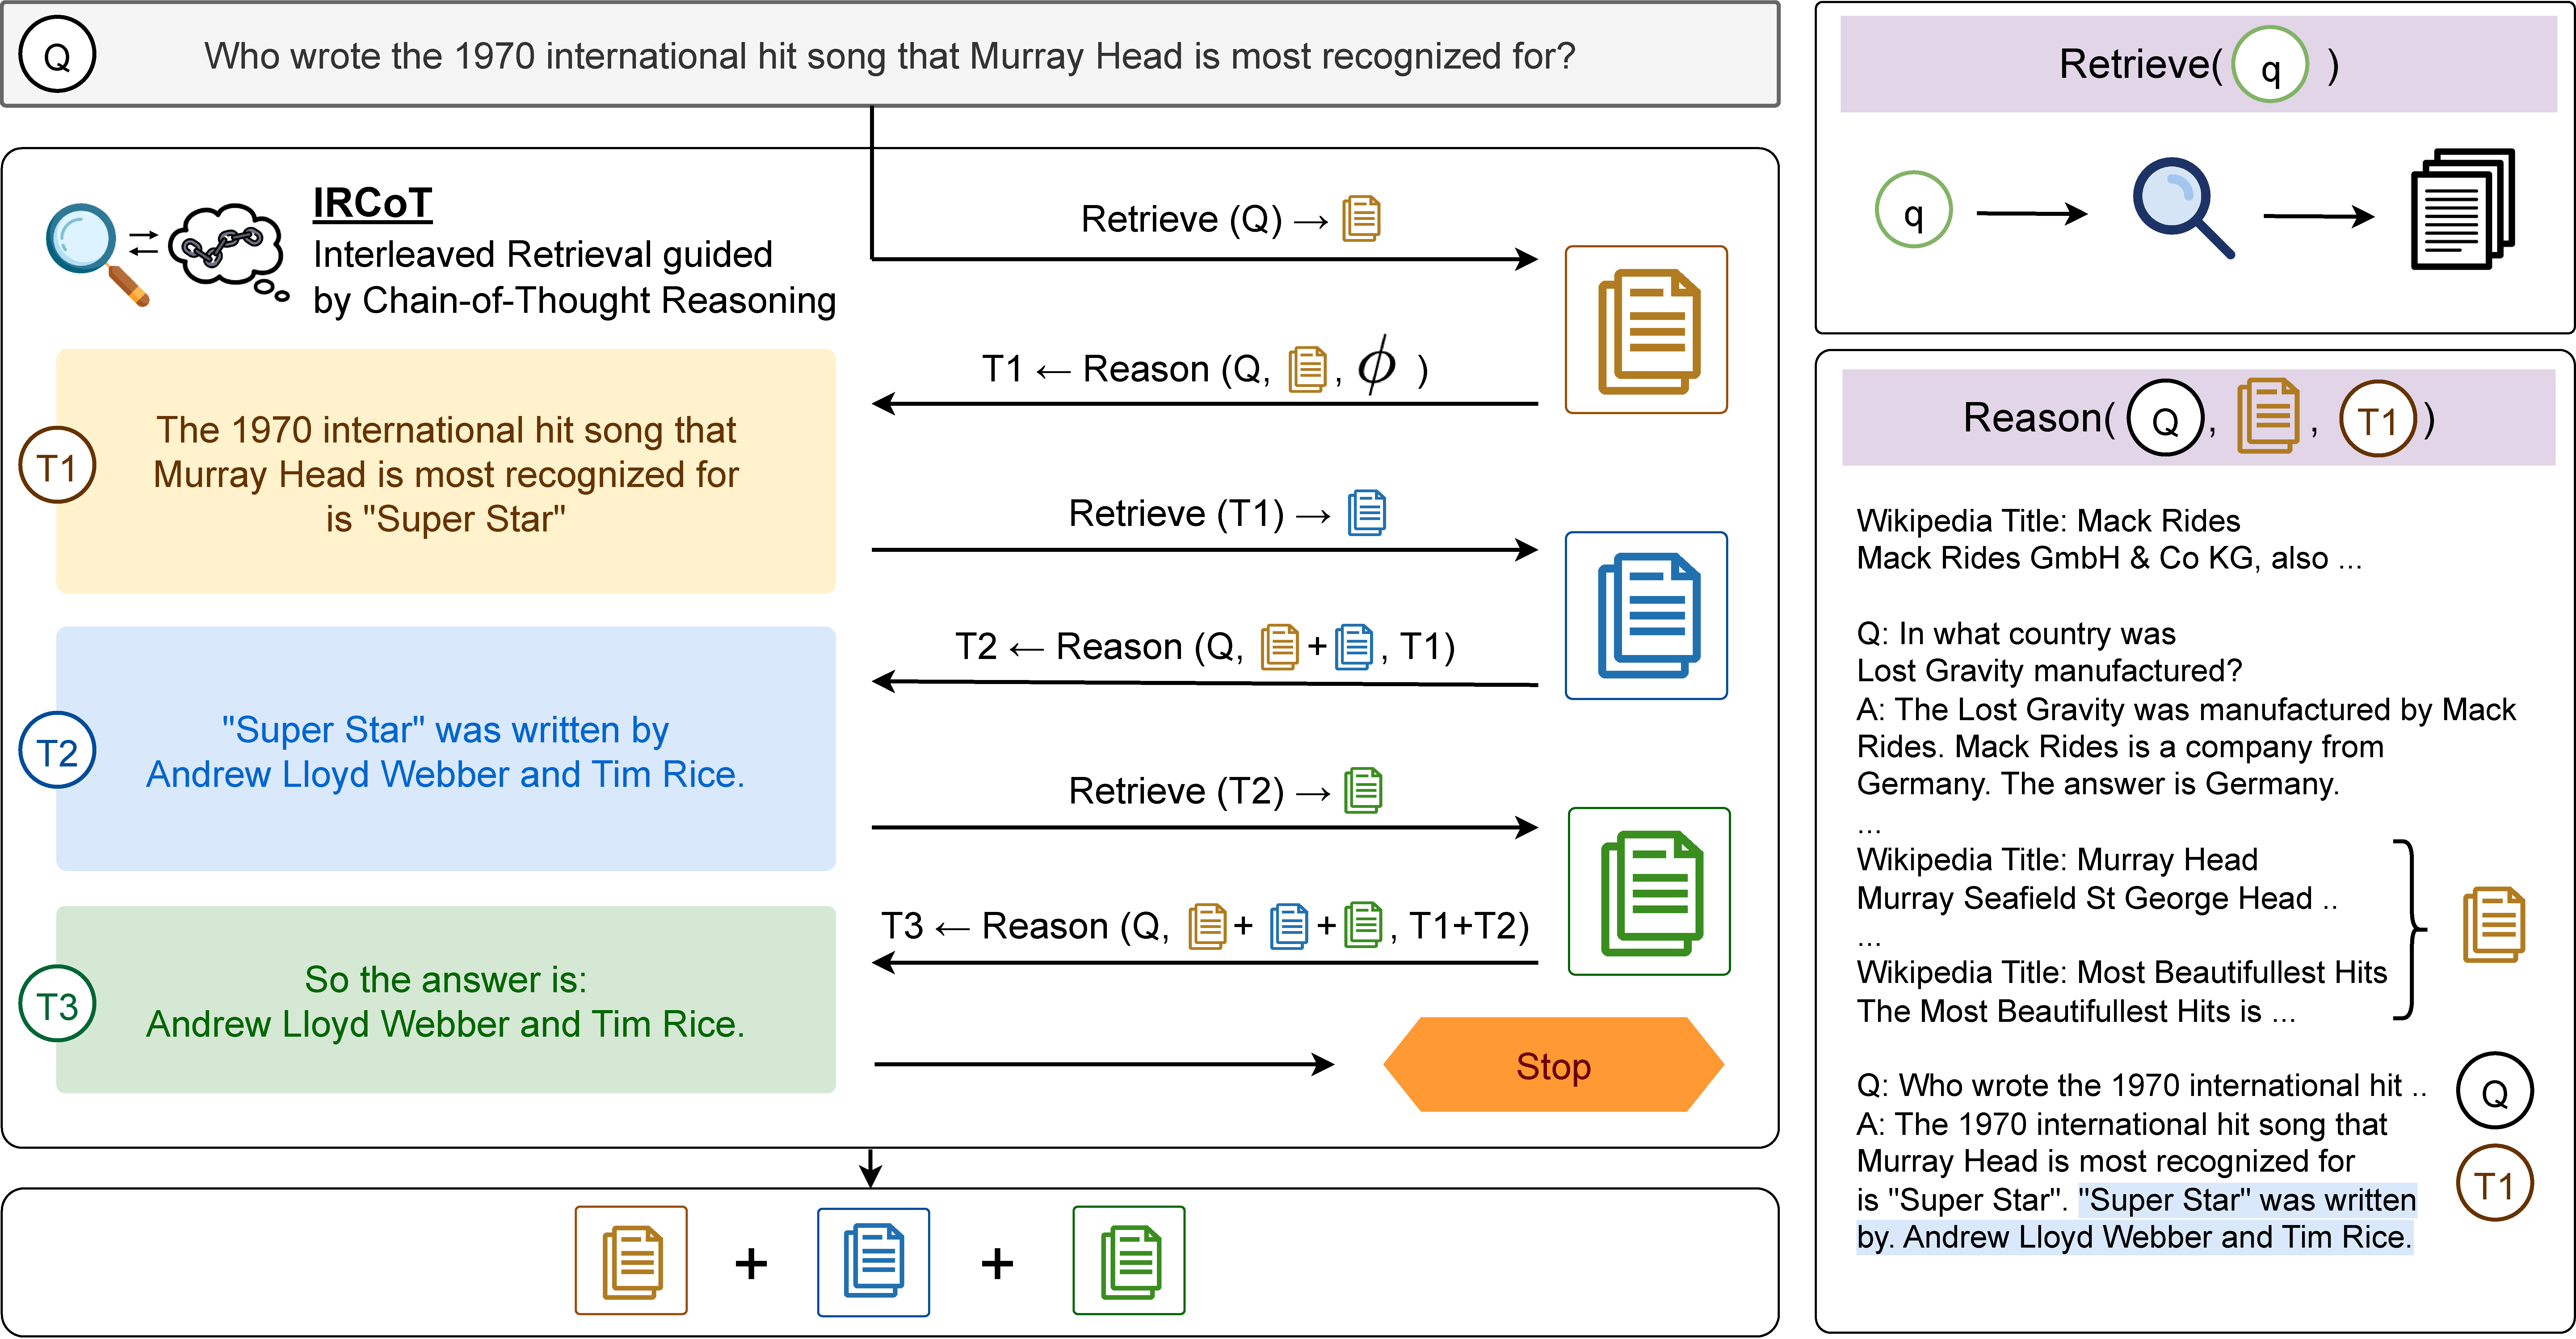
\includegraphics[width=0.95\textwidth]{images/main-figure.pdf}
\caption{\iconsys interleaves chain-of-thought (CoT) generation and retrieval steps to guide the retrieval by CoT and vice-versa. We start by retrieving $K$ documents using the question as they query and repeat two steps alternatingly until termination. (i) \texttt{reason}-step generates next CoT sentence based on the question, so far retrieved paragraphs, and CoT sentences. (ii) \texttt{retrieve}-step retrieves $K$ more paragraphs based on the last CoT sentence. The process terminates when the generated CoT has ``answer is'' or the number of steps exceeds a threshold. The collection of all paragraphs is returned as the retrieval result on the termination.}
\label{fig:main-figure}
\end{figure*}

Our goal is to answer a knowledge-intensive multi-step reasoning question $Q$ in a few-shot setting by using a knowledge source containing a large number of documents. To do this we follow a \texttt{retrieve-and-read} paradigm~\cite{retrieve-and-read}, where the retriever first retrieves documents from the knowledge source and the QA model reads the retrieved documents and the question to generate the final answer. Our contribution is mainly in the \texttt{retrieve} step (\S\ref{subsec:retriever}), and we use standard prompting strategies for the \texttt{read} step (\S\ref{subsec:reader}).

As noted earlier, for multi-step reasoning, retrieval can help guide the next reasoning step, which in turn can inform what to retrieve next. This motivates our interleaving strategy, discussed next.

\subsection{Interleaving Retrieval with Chain-of-Thought Reasoning}
\label{subsec:retriever}

Our proposed retriever method, \iconsys, can be instantiated from the following three ingredients: (i) a base retriever that can take a query and return a given number of paragraphs from a corpus or knowledge source; (ii) a language model with zero/few-shot Chain-of-Thought (CoT) generation capabilities; and (iii) a small number of annotated questions with reasoning steps explaining how to arrive at the answer in natural language (chain of thoughts) and a set of paragraphs from the knowledge source that collectively support the reasoning chain and the answer.

The overview of \iconsys is given in Fig.~\ref{fig:main-figure}. We first gather a base set of paragraphs by retrieving $K$ paragraphs using the question $Q$ as the query. Then, we interleave two steps (\texttt{reason} and \texttt{retrieve}) iteratively until the termination criterion is met.

The \textbf{retrieval-guided reasoning step (``Reason'')} generates the next CoT sentence using the question, the paragraphs collected thus far, and the CoT sentences generated thus far. The prompt template for the task looks as follows:

\begin{small}
\begin{verbatim}
Wikipedia Title: <Page Title>
<Paragraph Text>
...
Wikipedia Title: <Page Title>
<Paragraph Text>

Q: <Question>
A: <CoT-Sent-1> ... <CoT-Sent-n>
\end{verbatim}
\end{small}
 
For in-context demonstrations, we use the complete CoT in the above format. For a test instance, we show the model only the CoT sentences generated thus far and let it complete the rest. Even though the model may output multiple sentences, for each \texttt{reason-step}, we only take the first generated sentence and discard the rest.

For the paragraphs in the in-context demonstrations, we use ground-truth supporting paragraphs and $M$ randomly sampled paragraphs shuffled and concatenated together in the above format. For a test instance, we show all the paragraphs collected thus far across all the previous \texttt{retrieve-step}s.

If the generated CoT sentence has the ``answer is:'' string or the maximum number of steps\footnote{set to 8 in our experiments.} has been reached, we terminate the process and return all collected paragraphs as the retrieval result.

The \textbf{CoT-guided retrieval step (``Retrieve'')} uses the last generated CoT sentence as a query to retrieve more paragraphs and adds them to the collected paragraphs. We cap the total number of collected paragraphs\footnote{set to 15 in our experiments.} so as to fit in at least a few demonstrations in the model's context limit.


\subsection{Question Answering Reader}
\label{subsec:reader}

The QA reader answers the question using retrieved paragraphs taken from the retriever. We consider two versions of the QA reader implemented via two prompting strategies: \texttt{CoT Prompting} as proposed by \citet{cot}, Direct Prompting as proposed by \citet{originalgpt3}. For CoT prompting, we use the same template as shown in \S\ref{subsec:reader}, but at test time we ask the model to generate the full CoT from scratch. The final sentence of CoT is expected to be of the form ``answer is: ...'', so that the answer can be extracted programmatically. If it's not in that form, the full generation is returned as the answer. For Direct Prompting, we use the same template as CoT Prompting but the answer field (``A: '') contains only the final answer instead of CoT. See App.~\ref{sec:apndx-prompts} for details.
